\section{Studi Pemilihan Umum di ABM}

\lettrine[nindent=-0.01em,findent=0.2em]{M}{etode} ABM sangat ampuh digunakan dalam memodelkan permasalahan sehari-hari karena dapat memodelkan masalaah tanpa melibatkan banyak proses matematika yang rumit \cite{crooks2018agent}. Pemilihan pemim-pin menjadi salah satu contoh masalah yang dapat dimodelkan di ABM. Munculnya sistem pemerintahan yang demokrasi membawa semakin banyak pihak yang terlibat dalam proses pembuatan keputusan dan memperbanyak variabel dalam menghitung peluang para calon untuk dapat memenangkan pemilihan \cite{feddersen2004rational}, terutama perilaku setiap orang dan interaksi didalamnya sangat berpengaruh terhadap hasil dari pemilihan. Banyak penelitian dilakukan untuk masalah pemilihan (voting) ini \cite{feddersen2004rational,saaty1989group}. Dalam skala kecil, masalah voting bisa hanya permasalahan membagi sekelompok murid ke dalam dua tim yaitu  merah dan biru, tetapi dalam masalah yang lebih besar dapat dikaitkan pada pemilihan presiden atau pemilihan pemimpin serikat negara. Kasus pemilihan pemimpin ini dapat diselesaikan menggunakan ABM dimana para pelaku pemilih dipandang sebagai agen-agen yang berperan didalamnya. Background dari agen dan cara berinteraksi dapat dijadikan sebagai dasar  dari aturan interaksi dalam membangun model dari pemilihan \cite{kazil2020utilizing}.

Banyak hal yang mempengaruhi setiap individu dalam melakukan pemilihan atau bahkan memilih untuk tidak memilih. Dalam artikel \cite{olson2012logic} terdapat konsep rasionalitas instrumental, yang menurutnya individu rasional membuat pilihan yang mereka yakini akan membawa hasil yang paling mereka sukai, Olson berpendapat bahwa ada sedikit insentif rasional bagi individu untuk berkontribusi pada produksi barang publik (atau umum), mengingat mereka (para calon) yang mengeluarkan biaya, para pemilih akan tetap memperoleh benefit terlepas dari ikut berkontribusi (suara) atau tidak \cite{savigny_2014}. Pandangan ini meningkatkan jumlah pemilih yang memilih untuk tidak memilih (golput) pada acara pemilihan.

Pada tahun 2019, di Indonesia melakukan pemilihan umum baik legislative maupun presiden. Menurut tim Lembaga Survey Indonesia (LSI), mereka menyatakan bahwa jumlah golput untuk pemilihan presiden di tahun 2019 yaitu sekitar 19.24\% yang telah menurun dibandingkat Pilpresa sebelumnya di tahun 2014 yang mencapai 30.42\% \cite{bbc_2019}. Presentase tersebut sangatlah tinggi sehingga banyak usaha yang dilakukan untuk meningkatkan minat pemilih untuk ikut berpartisipasi melalui berbagai cara, baik itu melalui hadiah dan promo bagi yang telah melakukan kewajibannya untuk memilih hingga ancaman bila tidak berpartisipasi.

Melakukan pemilihan sebenarnya adalah reaksi rasional dari setiap individu \cite{feddersen2004rational}. Salah satu hal yang banyak dilakukan adalah dengan menempatkan aktor-aktor strategis yang dapat mengarahkan pemikiran secara rasional dari individu untuk melakukan pemilihan. Dalam pemilihan pendahuluan, ada bukti bahwa pemilih mengkondisikan pilihan suara mereka pada kelayakan kandidat \cite{abramson1992sophisticated}. Dalam sebuah studi komprehensif, penulis \cite{cox1997making} menunjukkan bahwa pola pemungutan suara dan hasil pemilu secara umum konsisten dengan pola perilaku yang diprediksikan oleh model voting strategis, misalnya di bawah aturan pluralitas (di mana kandidat dengan suara terbanyak memenangkan pemilihan).

Agen-agen strategis yang diterapkan pada penelitian ini adalah agen bayaran. Dalam hal ini, agen bayaran akan bertugas untuk mempengaruhi agen lain untuk mengikuti pilihan dari agen bayaran tersebut. Sehingga secara rasional para agen pemilih mengalami kenaikkan kecenderungan untuk mengikuti agen pemilih bayaran memilih pilihan. Model ini akan memperlihatkan bagaimana jumlah pemilih bayaran dapat berpengaruh dan bagaimana sekelompok kecil pemilih bayaran bila berada di posisi yang tepat akan mempercepat agen-agen pemilih untuk menentukan pilihannya.

Model pemilihan umum telah banyak diteliti baik di Indonesia maupun di dunia \cite{abramson1992sophisticated,cox1997making,wijayati2020money}. Untuk membangun model agen bayaran dalam pemilihan umum pemimpin, dimulai dengan model sederhana yaitu model voting yang terdapat pada NetLogo \cite{wilensky1999netlogo}, lalu model standing ovation yang dikembangkan oleh Miller dan Page \cite{miller2004standing}, dan seiring dengan meningkatnya komputasi untuk melakukan pemodelan, muncul MESA yang dikembangkan dengan bahasa Python \cite{kazil2020utilizing}. Model ini diharapkan dapat menggambarkan situasi pemilihan umum dengan banyak faktor yang mempengaruhi perilaku para pemilih. Salah satu yang akan ditekankan pada model ini adalah perilaku pemilih yang bergerak karena adanya aktor-aktor strategis yang menjadi gambaran seorang agen bayaran yang selanjutnya akan meningkatkan jumlah suara pemilih dan mempengaruhi hasil akhir dari pemilihan.

\subsection{Model Voting dari modul library NetLogo}

Untuk model pemilihan sebagai model paling sederhana dapat dilihat pada model voting yang disediakan oleh modul libraries Netlogo dan juga model standing ovation yang telah dikembangkan. Pada model voting, opini para agen akan terlihat dengan bagaimana setiap agen menentukan pilihannya berdasarkan observasi terhadap neighbours atau sekitarnya. Menurut penulis \cite{viridi2019agent} agen menempati satu sel grid yang lalu bergerak mengikuti pola yang ditetapkan.

Untuk memahami kestabilan suatu grup, model perlu diperbesar untuk mengurangi cluster dan  dan memahami konfigurasi saat dia stabil. Sebagai contoh, saat suatu sel dikelilingi (4 biru dan 4 hijau) disekitarnya maka posisi sel tersebut tidak akan berubah lagi. Meski demikian, hal ini tidak mudah bagi kita untuk memprediksi initial set dari suatu sel dan dimana batasnya hingga akhirnya kestabilan tercapai.

Dalam membagun model voting ini, digunakan aturan sederhana diantaranya sebagai berikut:

\begin{itemize}
	\item Bila neighbours menunjukkan jumlah opini seri, maka sel akan tetap pada pilihan terakhir dan tidak berubah lagi seterusnya

	\item Agen akan selalu mengikuti pilihan dari mayoritas dari agen-agen disekitarnya
\end{itemize}

\subsection{Model Standing Ovation Problem (SOP)}

Model standing ovation pertama kali dikenalkan oleh Miller dan Page (2004) dengan mengilustrasikan masalah pengambilan keputusan, yaitu bagaimana para penonton pada akhirnya akan ikut berdiri dan bertepuk tangan. Pada situasi tersebut, setiap penonton perlu memutuskan apa dia akan ikut berdiri atau tetap duduk diam. Tetapi, hal tersebut akan berubah bilamana dia dikekelingi oleh orang-orang yang berdiri dan bertepuk tangan. Hal ini terjadi secara alami untuk menghindari perasaan tidak nyaman karena berbeda dengan orang lain. Sama halnya dengan tidak mungkin seseorang merasa nyaman berdiri dan bertepuk tangan di saat semua orang duduk terdiam.

Pada model Miller dan Page, Terdapat sebuah auditorium berukuran $L \times L$ yang sesak dipenuhi oleh agen. Di akhir pertunjukkan, penonton akan mengevaluasi pertunjukkan berdasarkan dari jumlah tepuk tangan. Nilai persepsi dari agen $i$ merupakan nilai floating poin acak $\left( 0.1 \right) $ yang disebut $qi$ dan model ini ditentukan nilai batas sebesar $\left( 0.5 \right)$ apabila $qi > 0.5$.

Pada langkah selanjutnya, agen akan meninjau sekelilingnya jika sekelilingnya menunjukkan perilaku yang berbeda maka agen dapat merubah keputusannya. Model Miller dan page membuat dua jenis environment yaitu lima tetangga dan kerucut.

\begin{itemize}
	\item Pada skenario empat tetangga, agen akan memperhatikan agen yang berada di samping kanan, kiri, depan, dan belakang seperti Table \ref{tbl:formasi_sop}.

	\begin{table}[H]
		\centering
		\begin{tabular}{|c|c|c|}
			\hline
			F & \cellcolor{gray!30}F & F \\
			\hline
			\cellcolor{gray!30}F & \cellcolor{gray!50}X & \cellcolor{gray!30}F \\
			\hline
			F & \cellcolor{gray!30}F & F \\
			\hline
		\end{tabular}
		\caption{Formasi empat tetangga}
		\label{tbl:formasi_sop}
	\end{table}

	\item Pada skenario kerucut, agen akan melihat agen lain di sisi kanan dan kirinya, lalu tiga agen di baris pertama depan dan lima agen di baris kedua depan dan seterusnya seperti Tabel \ref{tbl:formasi_kerucut}.

	\begin{table}[H]
		\centering
		\begin{tabular}{|c|c|c|c|c|c|c|}
			\hline
			\cellcolor{gray!30}F & \cellcolor{gray!30}F & \cellcolor{gray!30}F & \cellcolor{gray!30}F & \cellcolor{gray!30}F & \cellcolor{gray!30}F & \cellcolor{gray!30}F \\
			\hline
			F & \cellcolor{gray!30}F & \cellcolor{gray!30}F & \cellcolor{gray!30}F & \cellcolor{gray!30}F & \cellcolor{gray!30}F & F \\
			\hline
			F & F & \cellcolor{gray!30}F & \cellcolor{gray!30}F & \cellcolor{gray!30}F & F & F \\
			\hline
			F & F & \cellcolor{gray!30}F & \cellcolor{gray!50}X & \cellcolor{gray!30}F & F & F \\
			\hline
		\end{tabular}
		\caption{Formasi kerucut}
		\label{tbl:formasi_kerucut}
	\end{table}
\end{itemize}

Ada aturan sederhana yang diterapkan di model standing ovation, yaitu:
\begin{enumerate}
	\item \textbf{Synchronous updating} (SU) :Semua agen memperbaharui statusnya secara bersamaan di waktu yang sama.

	\item \textbf{Asyncronous-random updating} (ARU): Pada setiap waktu setiap agen mereview mereka dengan urutan random
\end{enumerate}

\subsection{Model Pemilihan Umum SOP dengan menggunakan NetLogo}\label{sec:sbab_c}

Model pemilihan umum di SOP dapat dibagi menjadi dua bagian, sebagai berikut:

\subsubsection{Model Sederhana}

Pada tahap ini, pemodelan perilaku pemilih dalam pemilu dengan menggunakan pendekatan SOP (Standing Ovation Problem) akan dilakukan. Dalam pemodelan ini, digunakan asumsi sistem pemilihan umum bersifat terbuka dan perasaan (\textit{threshold}) dari setiap pemilih serta perilaku pemilih lainnya akan mempengaruhi perilaku seorang pemilih.

Dengan menggunakan pendekatan bottom-up, model dibuat sederhana yang mewakili entitas utama dalam sebuah pemilihan umum, yaitu Pemilih, kualitas kampanye serta variable lain yang bisa mempengaruhi keputusan pemilih. Agen yang digunakan dalam model ini hanya satu yaitu Pemilih sedangkan environment yang digunakan bersifat statis dan tidak mempunyai interaksi dengan dengan agent maupun dengan environment lainnya.

Agen mempunyai interaksi dengan agen lainnya dan dapat berubah perilakunya berdasarkan kriteria dari parameter yang ditentukan.

Agen mempunyai rules yang sangat sederhana, yaitu agen berdiri (Standing) sebagai representasi dari setuju memilih apabila kualitas kampanye ditambah noise lebih besar dari threshold yang dimiliki. Threshold dari setiap pemilih akan berbeda-beda (random) dan mengikuti pola distribusi tertentu. Pada masyarakat yang mempunyai kesamaan latar belakang sosial serta preferensi yang sama (homogen) dapat digunakan pola distribusi threshold berupa Normal (dengan mean atau nilai rata-rata threshold dan simpangan) sedangkan pada masyarakat yang heterogen dengan berbagai latar belakang sosial berbeda dapat digunakan pola distribusi threshold Uniform.

Agen juga mempunyai rules lainnya, yaitu agen akan Standing untuk memilih apabila mayoritas pemilih menyatakan Standing atau memilih.

Keputusan seorang pemilih untuk Standing (memilih) dapat di formulasikan Persamaan \ref{eq:sop1}:

\begin{equation}
Q_{campaign} + noise \approx threshold
\label{eq:sop1}
\end{equation}

Dengan $Q_{campaign}$ merupakan kualitas kampanye dari calon atau kandidat, $threshold$ adalah perasaan pemilih merespon kampanye dari calon atau kandidat, dan $noise$ adalah nilai acak (\textit{random}) sebagai variable dinamis untuk mendekatkan formulasi dengan kejadian sebenarnya. Apabila $Q_{campaign} + noise < threshold$, maka pemilih tidak akan berdiri (\textit{Sitdown}), yang merupakan representasi tidak memilih calon atau kandidat tersebut.

Dengn menggunakan aturan sederhana tersebut diatas, model sederhana dapat digunakan untuk mendekati bagaimana perilaku pemilih dalam pemilihan umum dalam sebuah Algoritma \ref{alg:sop_sederhana} sebagai berikut:

\begin{algorithm}
\caption{Model sederhana}\label{alg:sop_sederhana}
	\begin{algorithmic}[1]
	\Procedure{InitModel}{}
		\State $Setup$
		\State $CreateAgent$
		\State $threshold \longleftarrow rand$ \Comment{Set threshold each person with specific distribution type}
		\State $person \longleftarrow sitdown$ \Comment{Set initial person sitdown}
	\EndProcedure

	\Procedure{Evaluate}{}\Comment{Calculate total standing}
		\If{$\dfrac{TotalStanding}{TotalPerson} \geq LIMIT$}
			\State $person \longleftarrow standing$ \Comment{set person with status sitdown to standing}
		\EndIf

		\Return $person$
	\EndProcedure

	\Procedure{ModelSederhana}{}
		\Require $InitModel$
		\Require $Evaluate$

		\For{$person=0$ to $person=n$}
			\State evaluate

			\If{$Q_{campaign} + noise \geqslant threshold$}
				\State $person \longleftarrow standing$
			\Else
				\State $person \longleftarrow sitdown$
			\EndIf
		\EndFor\label{simplemodelforloop}
	\EndProcedure
	\end{algorithmic}
\end{algorithm}

\subsubsection{Model Kompleks}

Model kompleks merupakan pengembangan lebih lanjut dari model sederhana. Model ini keputusan pemilih selain di pengaruhi oleh kualitas kampanye ($Q_{campaign}$), akan dipengaruhi juga oleh pemberian uang dari kandidat atau calon (\textit{money politics}). Dalam kehidupan nyata, praktik seperti ini sering diketahui dari pemberitaan dan analisa para praktisi pemilihan walaupun tidak ada bukti empirik yang dapat di rujuk karena hal tersebut tentu merupakan pelanggaran peraturan. Akan tetapi, hal ini merupakan suatu hal yang sudah menjadi rahasia umum. Dalam pengetahuan publik, \textit{money politics} tersebut akan sangat mempengaruhi dan seringkali menjadi faktor penentu yang menjadi preferensi pemilih. Dalam model komplek, uang yang diterima pemilih dari agen bayaran akan menurunkan personal threshold sehingga peluang pemilih untuk Standing (memilih) lebih tinggi.

Dalam model kompleks, ada beberapa tambahan parameter sebagai berikut:

\begin{itemize}
\item $N\_agen\_bayar$: Jumlah agen bayar yang akan melakukan pembagian uang kepada pemilih

\item $Modal$: Jumlah uang awal yang di miliki oleh setiap agen bayar

\item $Neighbor\_standing$ : jumlah minimal pemilih sekitar yang melaku-kan Standing (memilih), dari total 8 pemilih sekitar (neighbors) dan membuat pemilih berubah pikiran menjadi Standing (memilih)
\end{itemize}

\subsection{Model Pemilihan Umum SOP dengan menggunakan Python Mesa}

Pada dasarnya terdapat kesamaan antara pemodelan pemilihan umum SOP di \texttt{NetLogo} dengan yang dilakukan di \texttt{Mesa}. Dalam pemodelan ini, Terdapat dua kategori umum agen yaitu:

\begin{enumerate}
\item \textbf{Agen bayaran} merupakan individu atau dapat berupa sekelompok orang yang memiliki fungsi membagikan uang atau insentif kepada calon pemilih.

\item \textbf{Agen pemilih} merupakan sekelompok calon pemilih yang memiliki fungsi memilih calon pemimpin. Agen ini memiliki tiga kondisi yaitu \texttt{yakin memilih}, \texttt{ragu-ragu}, dan \texttt{yakin tidak memilih}. Memang pada dasarnya di model SOP, luaran dari model bersifat biner yaitu apakah 1 (\textit{standing}) atau 0 (\textit{sitdown}). Namun dalam artikel ini, nilai diantaranya dimasukkan untuk melihat perubahan yang akan terjadi pada keragu-raguan. Dalam pemodelan ini, tingkat keyakinan dalam pemilihan ditentukan dari nilai batas atau \textit{threshold}.
\end{enumerate}

Dalam penerapan model pemilihan umum dengan SOP, ada beberapa faktor yang mempengaruhi seperti yang sudah dijelaskan pada sub-bab \ref{sec:sbab_c} yaitu peforma atau kualitas kampanye calon pemimpin, \textit{noise} atau faktor internal yang tidak terduga, dan uang atau insentif. Ketiga faktor yang disebutkan dapat mempengaruhi secara umum keinginan atau \textit{threshold} calon pemilih untuk memilih calon pemimpin. Dengan demikian, pemodelan ini di \texttt{Mesa} menggunakan formula dibawah.

\begin{equation}
Q_{campaign} + noise \times insentive \approx threshold
\label{eq:sop_mesa}
\end{equation}

Berdasarkan Persamaan \ref{eq:sop_mesa} di atas dapat dijelaskan faktor yang dapat mempengaruhi sebagai berikut:

\begin{itemize}
\item Kualitas atau performa kampanye ($Q_{campaign}$) dari calon pemimpin merupakan faktor utama dalam pemodelan ini. Faktor ini sangat menentukan calon pemilih untuk menentukan sikap apakah ikut memilih (\textit{standing}), ragu-ragu, atau tidak memilih (\textit{sitdown}).

\item Noise diperlukan dalam pemodelan ini sebagai faktor internal yang dapat terjadi tanpa diduga. Apabila faktor ini sedang baik bagi calon pemilih maka noise bernilai positif, begitu juga sebaliknya noise akan bernilai negatif. Faktor ini dapat berupa kesehatan calon pemilih, tingkat kebahagiaan, atau lainnya.

\item Insentive atau uang menjadi faktor dalam studi kasus pemilihan umum dengan SOP ini. Uang diterima oleh pemilih melalui pemberian agen bayaran saat agen-agen tersebut bertemu. Uang yang diberikan oleh agen bayaran kemudian dikategorikan ke dalam tiga kelompok oleh calon pemilih yaitu \texttt{kecil}, \texttt{sedang}, atau \texttt{besar}.
\end{itemize}

\subsubsection{Aturan Sederhana}\label{sec:sbab_aturansederhana}

Untuk membangun model di ABM, diperlukan aturan-aturan sederhana. Secara umum, pemodelan SOP ini di \texttt{Mesa} melibatkan baik agen bayaran dan agen pemilih dapat bergerak secara acak. Memang berbeda dari pemodelan SOP \cite{miller2004standing} dimana agen-agen tidak bergerak, namun pemodelan pemilihan umum di lapangan melibatkan agen bayaran yang bergerak bebas tanpa dikoordinir dan begitu juga dengan agen pemilih dapat bergerak bebas. Pergerakan acak dari agen bayaran dilakukan ke delapan arah (\textit{Moore}) apabila dibuat dalam bentuk grid seperti Tabel \ref{tbl:formasi_moore} di bawah. Lain halnya dengan agen pemilih, pergerakan agen ini diberikan dua opsi dapat berupa \textit{Moore} atau \textit{Von Neuman} (seperti Tabel \ref{tbl:formasi_sop}) \cite{zaitsev2017generalized}. Opsi ini diberikan untuk melihat pengaruh dari batasan pergerakan dari agen pemilih.

\begin{table}[H]
		\centering
		\begin{tabular}{|c|c|c|c|c|}
		\hline
		\cellcolor{gray!10}G & \cellcolor{gray!10}G & \cellcolor{gray!10}G & \cellcolor{gray!10}G & \cellcolor{gray!10}G \\
		\hline
		\cellcolor{gray!10}G & \cellcolor{gray!30}F & \cellcolor{gray!30}F & \cellcolor{gray!30}F & \cellcolor{gray!10}G \\
		\hline
		\cellcolor{gray!10}G & \cellcolor{gray!30}F & \cellcolor{gray!50}X & \cellcolor{gray!30}F & \cellcolor{gray!10}G \\
		\hline
		\cellcolor{gray!10}G & \cellcolor{gray!30}F & \cellcolor{gray!30}F & \cellcolor{gray!30}F & \cellcolor{gray!10}G \\
		\hline
		\cellcolor{gray!10}G & \cellcolor{gray!10}G & \cellcolor{gray!10}G & \cellcolor{gray!10}G & \cellcolor{gray!10}G \\
		\hline
		\end{tabular}
		\caption{Formasi delapan tetangga}
		\label{tbl:formasi_moore}
	\end{table}

Disamping aturan pergerakan, agen pemilih diberikan aturan jarak observasi ke tetangga sekitar. Jarak terdekat adalah sebesar 1 satuan grid. Penggunaan jarak observasi ini merupakan bagian dari terapan pemodelan dengan SOP. Dengan menerapkan jarak observasi ini dapat memberikan pengaruh "pasif" terhadap keinginan memilih bahkan dengan ketika agen bayaran sudah tidak ada. Maksud dari pengaruh "pasif" adalah agen pemilih yang tadinya ragu-ragu atau memang yakin tidak memilih dapat berubah menjadi ikut memilih karena faktor dari tetangga sekitar dengan jarak pengaruh tertentu. Dalam rentang jarak tersebut akan diakumulasi sehingga pemilih lain di sekitar lebih besar dari $70\%$ maka calon pemilih tersebut ikut memilih (\textit{standing}).

Aturan lainnya adalah masing-masing agen juga ditambahkan aturan berkaitan dengan uang atau insentif seperti yang diformulasikan dalam Persamaan \ref{eq:sop_mesa}. Agen bayaran dibekali dengan uang sebagai modal awal dalam upaya mempengaruhi keputusan pilihan calon pemilih. Uang awal ini dapat diubah di aplikasi apabila ingin melakukan variasi simulasi. Dalam hal pembagian uang, agen bayaran bersifat homogen. Jumlah uang yang dikeluarkan memiliki besaran yang sama ke setiap agen pemilih dan ini menjadi \textbf{batasan} dalam pemodelan yang dilakukan. Bisa saja terjadi pembayaran yang bersifat heterogen, yaitu agen bayaran berlaku curang dalam mengeluarkan jumlah uang ke agen pemilih namun hal demikian tidak dilakukan. Agen bayaran akan pergi apabila uang yang dibagikan sudah habis. Dari sisi agen pemilih, uang menjadi masukan dan dapat mempengaruhi keputusan memilih. Pemberian uang dari agen bayaran akan ditransformasikan ke dalam bentuk kategori yang sudah disampaikan sebelumnya.

Masing-masing agen pemilih dalam model diberikan opsi di aplikasi bersifat homogen (agen pemilih memiliki kecenderungan karakter atau kebiasaan yang mirip) atau heterogen. Berdasarkan opsi ini, memberikan pengaruh terhadap \textit{threshold} awal calon pemilih apakah saat itu \texttt{yakin memilih}, \texttt{ragu-ragu}, atau \texttt{tidak memilih}. Disamping itu juga, opsi ini memberikan pengaruh terhadap variabel \textit{noise} dalam Persamaan \ref{eq:sop_mesa}.

\subsubsection{Alur Kerja dan Pemodelan di Mesa}\label{sec:sbab_alurkerja}

Secara garis besar, model dengan \texttt{Mesa} ini melibatkan alur dari data masukan pengguna, model, dan hasil. Alur ini dapat diilustrasikan seperti Gambar \ref{fig:flowsopabm} dibawah.

\begin{figure}[H]
\centering
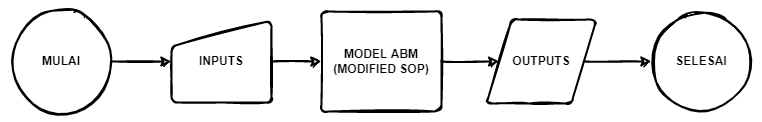
\includegraphics[width=\linewidth]{images/ch02/FlowSopAbm}
\caption{Diagram alir penerapan modifikasi model SOP}
\label{fig:flowsopabm}
\end{figure}

Saat pengguna mulai menjalankan aplikasi dengan  \texttt{Mesa}, bagian yang diperlukan pertama kali adalah \texttt{inputs}. Bagian ini terdiri dari peforma atau kualitas calon pemimpin, jumlah agen bayaran, jumlah pemilih, tipe pemilih, tipe tetangga, radius pengamatan pemilih, jumlah uang atau modal awal, dan jumlah uang yang dikeluarkan.

Peforma calon pemimpin diberikan rentang nilai 0.1 hingga 1 dengan nilai awal adalah 0.5. Peforma kampanye dinilai buruk jika bernilai minimum dan baik jika bernilai maksimum. Dalam pemodelan ini, jumlah agen bayaran memiliki rentang nilai 1 hingga 15 dengan nilai awal adalah 10. Untuk agen pemilih, rentang jumlah pemilih dari 50 hingga 350 dengan nilai awal adalah 100. Tipe pemilih memiliki dua opsi yaitu homogen dan heterogen serta jenis tetangga (\textit{neighbour}) ada dua yaitu \textit{Moore} (delapan arah) dan \textit{Von Neumann} (empat arah). Untuk agen bayaran dibekali sejumlah uang dengan rentang 100 hingga 1000 dengan nilai awal adalah sebesar 500. Terakhir, jumlah uang yang dikeluarkan dengan rentang dari 10 hingga 50 dengan nilai pengeluaran awal sebesar 25.

Selanjutnya adalah bagian proses modifikasi model pemilihan umum dengan SOP di ABM. Sudah dijelaskan sebelumnya bahwa model ini dibekali dengan aturan-aturan sederhana dan terdiri dari agen-agen bayaran dan pemilih. Untuk itu, model ini dibangun sesuai dengan Algoritma \ref{alg:modelagenbayaran} berikut ini \footnote{Untuk \textit{source code} dapat diakses di \url{https://github.com/akbarpn136/abm}}.

\begin{algorithm}[H]
	\caption{Model Agen Bayaran}\label{alg:modelagenbayaran}
	\begin{algorithmic}[1]
		\Procedure{AgenBayaran}{}\Comment{Modifikasi SOP untuk agen bayaran}
			\State $self.width \gets width$\Comment{lebar grid}
			\State $self.height \gets height$\Comment{tinggi grid}
			\State $self.peforma \gets peforma$
			\State $self.radius\_pengamatan \gets radius\_pengamatan$
			\State $self.pengeluaran\_uang \gets pengeluaran\_uang$
			\State $self.initial\_uang \gets initial\_uang$
			\State $self.initial\_agen\_bayaran \gets initial\_agen\_bayaran$
			\State $self.initial\_pemilih \gets initial\_pemilih$
			\State $self.initial\_tipe\_pemilih \gets initial\_tipe\_pemilih$
			\State $self.initial\_tipe\_tetangga \gets initial\_tipe\_tetangga$
			\\ \Comment{mulai membuat agen bayaran}
			\For{$i=0$ to $i=self.initial\_agen\_bayaran$}\label{balg:buatagenbayaran}
				\State $position \gets random\_range(self.width, self.heigth)$
				\State $bayaran \gets Bayaran(id,position,Moore,self.initial\_uang)$
				\State $grid.place\_agent(bayaran, position)$
			\EndFor

			\\ \Comment{mulai membuat agen pemilih}
			\For{$j=0$ to $j=self.initial\_pemilih$}\label{balg:buatagenpemilih}
				\State $position \gets random\_range(self.width, self.heigth)$\label{balg:posisiacakpemilih}
				\State $tipe\_tetangga \gets self.initial\_tipe\_tetangga == "Moore"$\label{balg:tipetetangga}
				\\
				\If{$self.initial\_tipe\_pemilih == "Homogen"$}\label{balg:pemilihankeinginan}
					\State $keinginan \gets random.uniform(0, 1)$
				\Else
					\State $keinginan \gets random.gauss(0.5, 0.4)$
				\EndIf
				\\
				\State $pemilih \gets Pemilih(id, position, tipe\_tetangga, keinginan)$
				\State $grid.place\_agent(pemilih, position)$
			\EndFor
		\EndProcedure
	\end{algorithmic}
\end{algorithm}

Memang tidak diragukan lagi bahwa agen bayaran dan pemilih ditempatkan pada posisi acak saat awal simulasi dimulai. Hal ini dapat dilihat dalam Algoritma \ref{alg:modelagenbayaran} pada baris \ref{balg:buatagenbayaran} dan \ref{balg:buatagenpemilih}. Untuk agen bayaran membutuhkan prosedur \texttt{Bayaran} seperti Algoritma \ref{alg:agenbayaran} dengan argumen-argumen yang sudah dijelaskan pada sub bab \ref{sec:sbab_aturansederhana}.

Untuk agen pemilih membutuhkan prosedur \texttt{Pemilih} seperti Algoritma \ref{alg:agenpemilih}. Prosedur \texttt{Pemilih} membutuhkan variabel pada baris \ref{balg:posisiacakpemilih}, \ref{balg:tipetetangga}, dan \ref{balg:pemilihankeinginan}.

\begin{algorithm}[H]
	\caption{Agen Bayaran}\label{alg:agenbayaran}
	\begin{algorithmic}[1]
		\Procedure{Bayaran}{id,position,moore,uang}
			\State $this\_cell \gets grid.get\_cell\_list\_contents([position])$
			\\
			\While{$loop \gets True$}
				\If{$isinstance(obj, Pemilih)$}\label{balg:periksajenisagen}
					\State $pemilih \gets append(obj)$\Comment{Simpan sebagai array pemilih}
				\EndIf
				\\
				\If{$len(pemilih)>0 \And pemilih.terima == False$}\label{balg:cekjumlahpemilih}
					\State $pemberian \gets pengeluaran\_uang$\Comment{beri uang ke pemilih}
					\State $self.uang -= pengeluaran\_uang$
				\EndIf
				\\
				\If{$self.uang \leq 0$}\label{balg:hapusagenbayaran}
					\State $grid.remove\_agent(self.position)$
				\EndIf
			\EndWhile
		\EndProcedure
	\end{algorithmic}
\end{algorithm}

Agen bayaran dibangun dengan aturan-aturan sederhana. Hal ini dikarenakan setiap gerakan acak agen ini melalui tahap pemeriksaan. Pemeriksaan pertama adalah pada baris \ref{balg:periksajenisagen}, ada kemungkinan agen bayaran bertemu dengan lebih dari satu agen pemilih. Apabila itu adalah agen pemilih makan agen bayaran menyimpan agen tadi kedalam kumpulan pemilih. Pada baris \ref{balg:cekjumlahpemilih}, apabila bertemu agen pemilih dan agen tersebut belum menerima uang pemberian maka uang akan diberikan ke agen tadi dan uang akan dikurangi dari modal agen bayaran. Aturan terakhir adalah pada baris \ref{balg:hapusagenbayaran} yaitu apabila uang agen bayaran sudah habis maka agen akan pergi.

\begin{algorithm}[H]
	\caption{Agen Pemilih}\label{alg:agenpemilih}
	\begin{algorithmic}[1]
		\Procedure{Pemilih}{id,position,moore,keinginan}
			\State $pemberian \gets 0$
			\State $terima \gets False$
			\State $thrsh \gets 0.8$\Comment{threshold}
			\State $radius \gets radius\_pengamatan$

			\While{$loop \gets True$}
				\If{$pemberian > True$}
					\State $terima \gets True$
				\EndIf
				\\
				\If{$pemberian \leq 10$}\label{balg:periksabesarpemberian}
					\State $skor \gets 0.01$
				\ElsIf{$10 < pemberian < 25$}
					\State $skor \gets 0.2$
				\Else
						\State $skor \gets 0.5$
				\EndIf
				\\
				\State $pemilih \gets grid.get\_neighbors(position, moore, radius)$\label{balg:tetanggapemilih}
				\State $jumlah\_individu \gets sum(map(keinginan \geq thrsh,pemilih))$\label{balg:lakukanakumulasipemilih}
				\State $homogenkah \gets initial\_tipe\_pemilih == "Homogen"$

				\If{homogenkah}\label{balg:ceknoisehomogen}
					\State $noise \gets random.uniform(-0.1, 0.1)$
				\Else
					\State $noise \gets random.gauss(0.0, 0.1)$
				\EndIf

				\If{$jumlah\_individu / len(pemilih) \geq 0.7$}\label{balg:hitungkeinginan}
					\State $keinginan += peforma + noise * skor$
				\EndIf
			\EndWhile
		\EndProcedure
	\end{algorithmic}
\end{algorithm}

Berdasarkan aturan sederhana dalam pemodelan pemilihan umum dengan SOP, agen pemilih dapat menerima uang atau insentif dari agen bayaran. Uang yang diterima ditransformasikan kedalam kategori sederhana seperti baris \ref{balg:periksabesarpemberian} yaitu $kecil=0.01$, $sedang=0.2$, dan $besar=0.5$. Pada baris \ref{balg:tetanggapemilih}, dilakukan dengan mengikuti konsep radius pengamatan di SOP dengan besar radius dengan rentang tertentu seperti yang sudah disampaikan sub bab \ref{sec:sbab_alurkerja}. Pada baris selanjutnya yaitu baris \ref{balg:lakukanakumulasipemilih} melakukan penjumlahan masing-masing agen dengan keinginan besar untuk memilih. Untuk perhitungan \textit{noise} dilakukan pada baris \ref{balg:ceknoisehomogen}. Apabila akumulasi tetangga sekitar lebih besar dari $70\%$ yakin memilih sesuai baris \ref{balg:hitungkeinginan} maka Persamaan \ref{eq:sop_mesa} dapat dilakukan. Jadi, apabila keinginan masing-masing agen pemilih lebih besar dari \textit{threshold} maka agen pemilih yakin untuk memilih.
